\documentclass[11pt]{article}
\usepackage{amsmath,textcomp,amssymb,graphicx,enumerate}
\usepackage{algorithm} % Boxes/formatting around algorithms
\usepackage[noend]{algpseudocode} % Algorithms
\usepackage{hyperref}
\hypersetup{
    colorlinks=true,
    linkcolor=blue,
    filecolor=magenta,      
    urlcolor=blue,
}

\usepackage[final]{style}
\usepackage[utf8]{inputenc}
\usepackage[T1]{fontenc}

\title{Lecture 16: Recognizing Objects by Parts}
\author{
  Tyler Dammann, Patrick Mogan, Qiqi Ren, Cody Stocker, Evin Yang \\
  Department of Computer Science\\
  Stanford University\\
  Stanford, CA 94305 \\
  \texttt{\{tdammann, pjmogan, qiqiren, cstock2, evin\}@stanford.edu} \\
}

\begin{document}
\maketitle
\section{Introduction}
One overarching goal of computer vision is to not only determine an object's class, but also relevant information about that object. Motivating examples include:
 \begin{itemize}
   \item Determining the number of calories in a sushi using its image?
   \item Using the image of a tiger to identify the safest course of actio?
   \item Given a chair, can we find out where we can buy it online?
   \item using computer vision and images of mushrooms to identify if they are edible?
 \end{itemize}
In general, computer vision should be able to give helpful information about an object beyond just basic characteristics.
\section{What can computers recognize today?}
Computer vision algorithms can easily detect and recognize faces in images.\\ \\
Object identification software such as Google Goggles can find very specific kinds of objects (e.g. logos, landmarks, books, text, contact info, and artwork), but can only find exact matches. Finding a generic object is much harder for today's systems.
\section{What's next to work on?} 
A principle milestone in computer vision yet to be reached is universal class recognition. That is, we would like an algorithm that could, for an image of any object, identify its class.
Examples include:
\begin{itemize}
	\item For an image of an orange mug, we would like coffee mugs to be the result, but image search found similar images by looking for something orange in the center – not mugs.
    \item Given an image of someone with a gas pump, we'd like to recognize that the gas pump is in the picture, but Google image search gives us images of people standing in same area of picture, maybe wearing the same color clothing.
    \end{itemize}
The PASCAL VOC challenge$^1$ taught models how to classify 20 classes of objects.
However, a particular model can only recognize a finite number of object classes. A model cannot recognize an arbitrary object, such as a coffee mug, if it is outside the model's set of training classes. We want to be able to recognize everything, but there are a lot of ``things'', and the agreed-upon number of ``things'' is increasing over time, so it is hard to decide which ones to focus on. In addition, there is not even an agreed-upon number of ``things'' in the universe -- there are 60K+ product categories on eBay, 80K+ English nouns on WordNet, 3.5M+ unique tags on Flickr, and 4.1M+ articles on Wikipedia.\\
\section{Big Data from the Internet}
Because of the sheer amount of available data, the Internet should be able to teach us a huge number of things. Internet traffic has been steadily increasing, and vast majority (86\%) is visual data. \\
\begin{figure}[h]
  \centering
  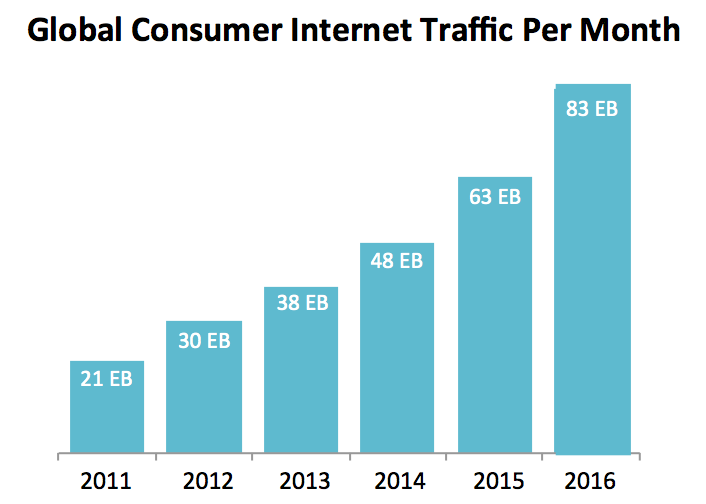
\includegraphics[scale=0.6]{internettraffic.png}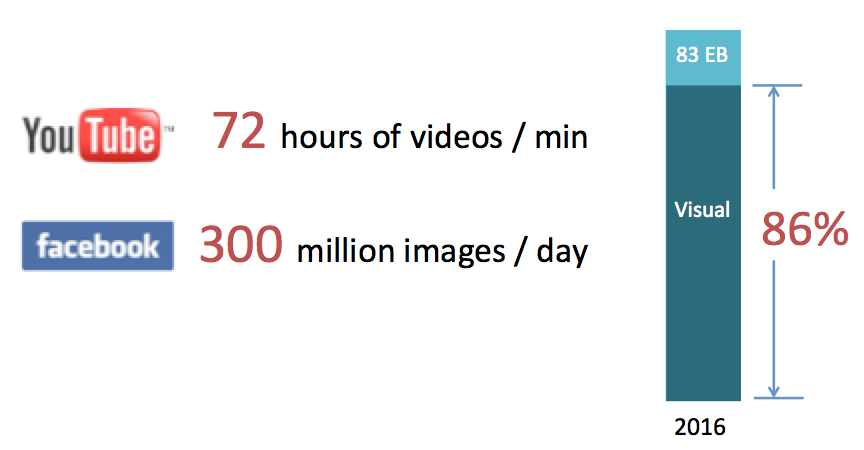
\includegraphics[scale=0.6]{fbyoutubedata.png}
  \caption{ Global Internet Traffic. Source: Lecture 16}
\end{figure}\\
Visual data is known as the dark matter of the Internet because we can't autoclassify or auto-analyze it. Trying to categorize a photoshopped ``pitbullfrog'' shows that machines struggle to generalize, improvise, and extrapolate with the ease that humans do. Thus, images are not enough; just as important is leveraging the crowd, which can provide answers to questions that machines would otherwise have difficulty tackling themselves, such as in the following example:\\
\begin{figure}[h]
  \centering
  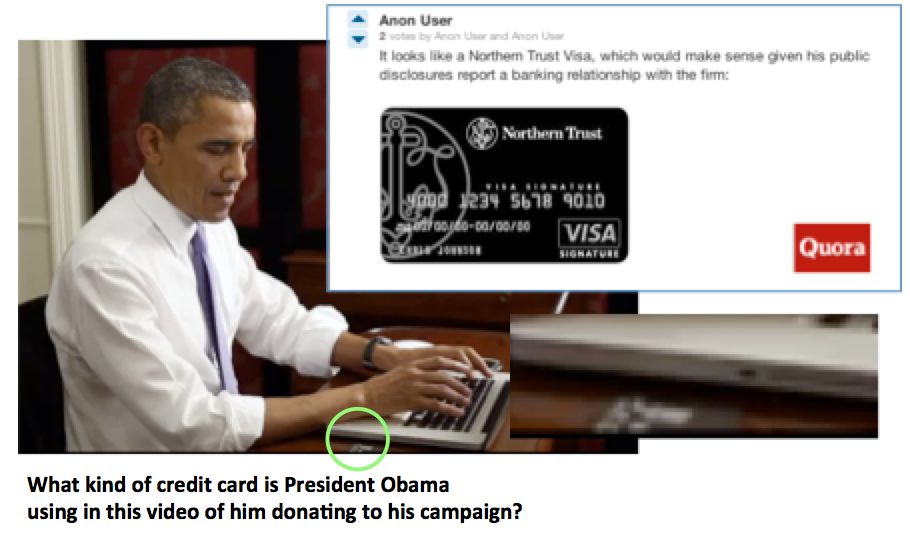
\includegraphics[scale=0.6]{obamacreditcard.png}
  \caption{Example Image Recognition Problem. Source: Lecture 16}
\end{figure}\\
Vitally, behind the big data is all of the users who are contributing their domain knowledge. When an individual cannot find the answer to a problem, it is easy to find others that can help. Image recognition systems, on the other hand, do not necessarily achieve this right now. The Internet gives an environment in which these two resources can be combined.
\section{ImageNet and Confusion Matrices}
Since models are limited by the number of the classes in the training set, one possible method of advancing universal class recognition is to create datasets with many more than the 20 classes the PASCAL VOC provided. \\ \\
ImageNet is a large image database created by Jia Deng in 2009 that  has 22,000 categories and 14 million images. It has become so important to computer vision that most projects now train on ImageNet before tackling other challenges. Other well-known databases include: Caltech101 (9K images, 101 categories), LabelMe (30k images), SUN (131K images).\\ \\
Deng applied four top classification methods from PASCAL VOC to ImageNet, but found that increasing the number of categories on which the models trained decreased their accuracy greatly. He plotted his findings as the following confusion matrix: \\
\begin{figure}[h]
  \centering
  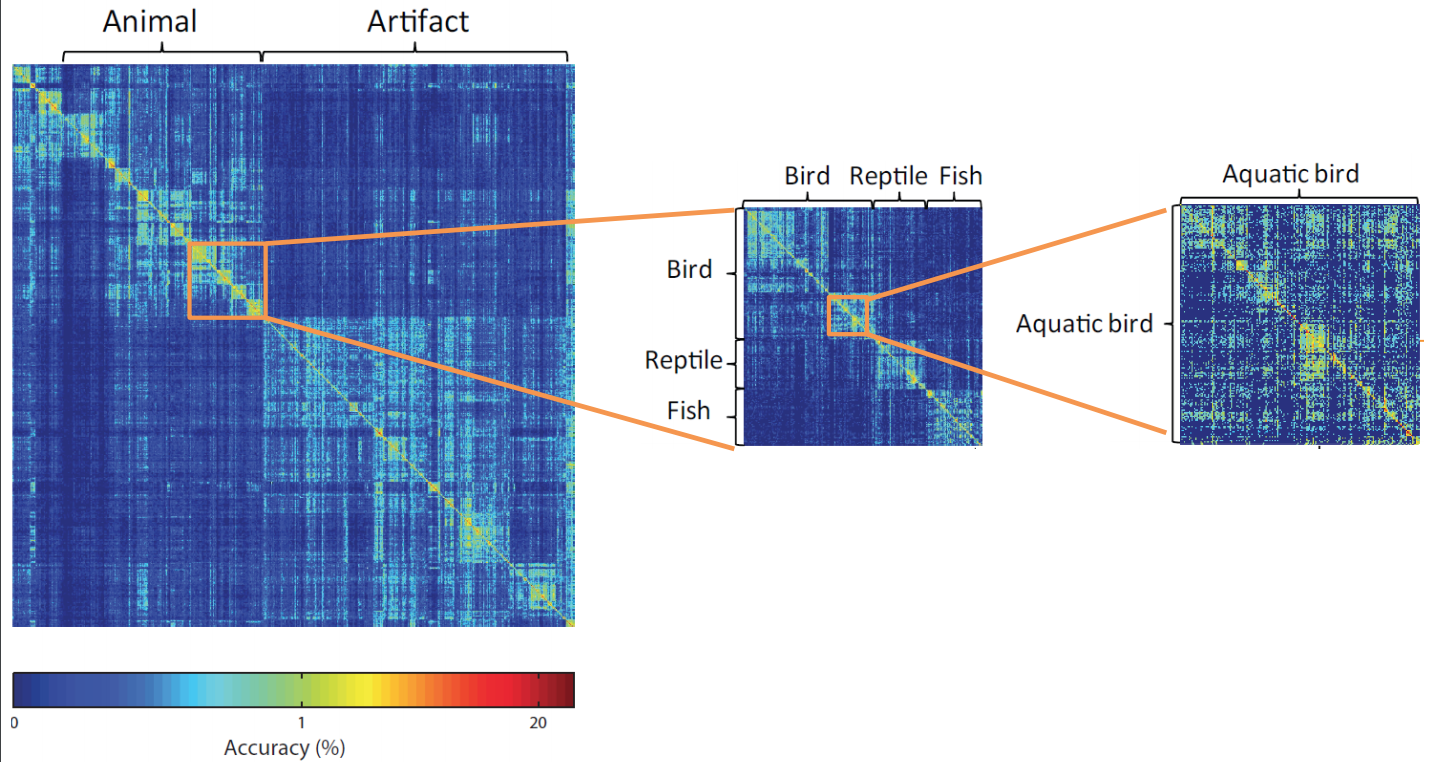
\includegraphics[scale=0.6]{confusionmatrix.png}
  \caption{ImageNet Confusion Matrix. Source: Lecture 16}
\end{figure}\\
A confusion matrix plots categories on the x and y axis and measures the degrees to which objects in a category are correctly or incorrectly classified. If we had a perfect detector, the only bright areas would be along the center diagonal line; this means everything is correctly classified (i.e., no misclassification).\\ \\
We see from this matrix that models are more prone to making classification errors when presented with items whose categories are very similar; for example, models struggle with discerning between different types of aquatic birds, while it can more easily categorize birds versus dogs. In other words, distinguishing between ``fine-grained'' categories is very difficult, since the distance between those categories is much smaller than between larger categories.
\section{Challenges and Solutions}
\subsection{Semantic Hierarchy}
\begin{figure}[h]
  \centering
  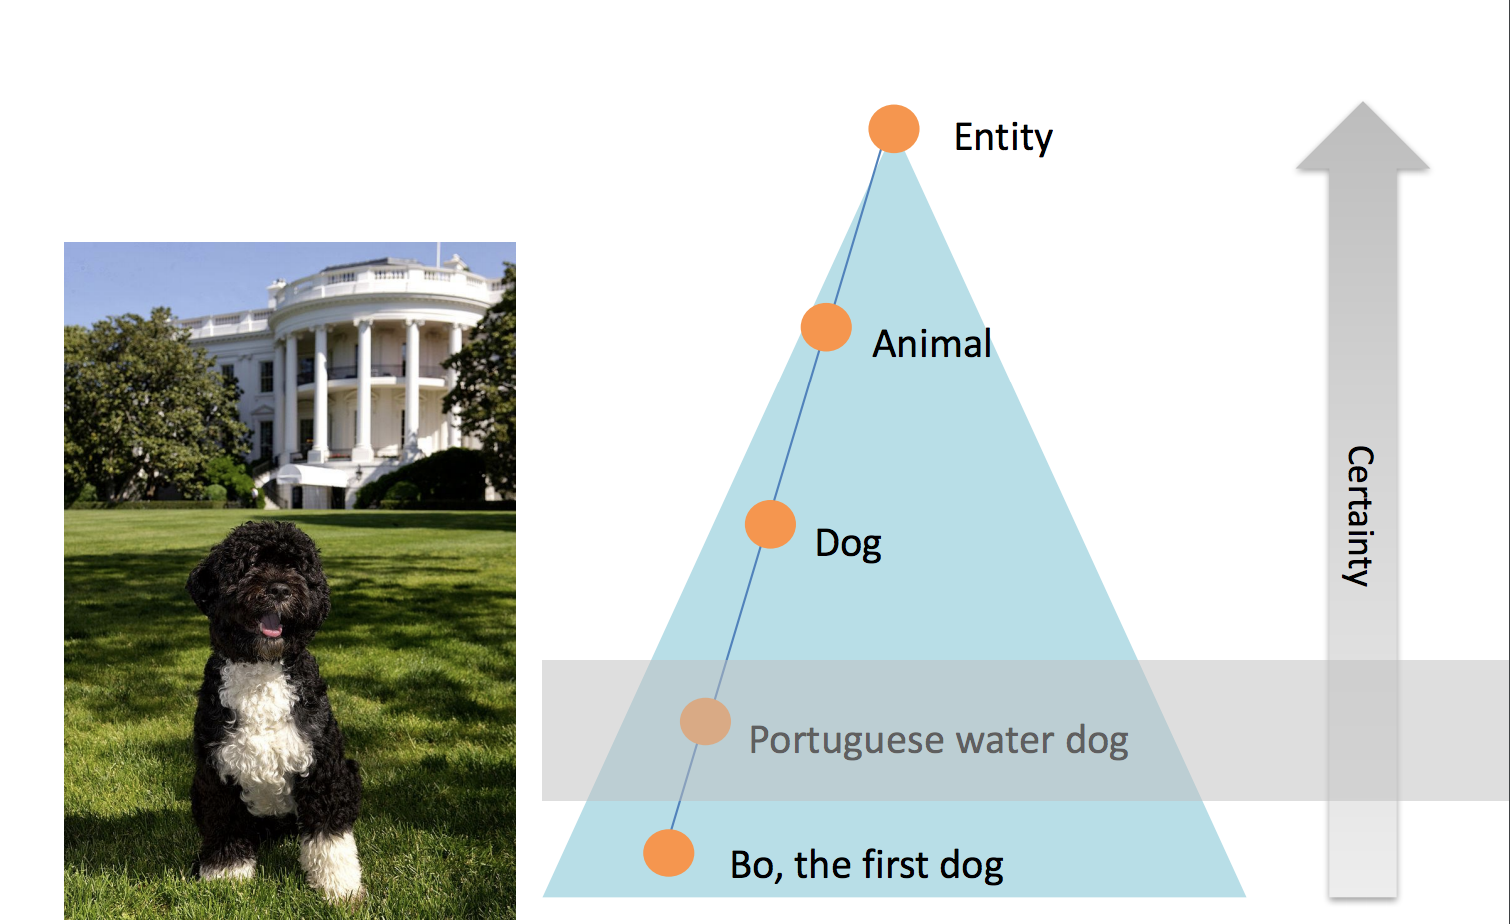
\includegraphics[scale=0.6]{bo.png}
  \caption{Example Semantic Hierarchy. Source: Lecture 16}
\end{figure}
One method for solving the issue of correctly classifying similar classes without making wrong guesses is the idea of a ``semantic hierarchy''. An example can be seen in Figure 4. Essentially, a tree is created, where every child is a more specific subclass of the parent. As the category gets more specific, uncertainty increases. The system will attempt to be as specific as possible (as low down on the tree as possible) without an unacceptable probability of misclassifying the object. This concept is called ``hedging'' - the system tries to identify where in the uncertainty tree to make a guess such that it is as informative as possible with few mistakes.\\ \\ 
To formally define this problem, we will assume that the training and test set have the same distribution. In addition, we will assume that we have access to a base classifier $g$ that gives a posterior probability on the hierarchy. We then define a reward function $R(f)$. We make $R(f)$ to have higher values at points farther down the hierarchical tree (when it classifies objects more specifically). Then, we also define an expected accuracy function $A(f)$. This function decreases as we move down the tree (since we are less certain about more specific guesses). Our problem statement is then to maximize $R(f)$ subject to the constraint that $A(f) \ge 1 - \epsilon$, where $\epsilon$ is a predetermined constant that represents the allowable error of our classifier over all of our examples.\\ \\
However, potential non-optimal solutions (in terms of $R(f)$) can arise given this method. In order to fix this, we can define a global, fixed, scalar parameter $\lambda \ge 0$. For each node, we add $\lambda$ to the reward value of that node, then normalize the posterior distribution. The process is then as follows:
\begin{enumerate}
\item Pick a $\lambda$.
\item Find the decision rule $f$ with $\lambda$.
\item Measure the performance on the validation set.
\item Check if $A \approx 1 - \epsilon$. Repeat from step one if necessary. 
\end{enumerate}
We can use binary search to find the best $\lambda$ quickly.\\
\subsection{Fine-grained Classes}
Existing work selects features from all possible locations in an image, but it can fail to find the right feature. For example, the difference between the Cardigan Welsh Corgi and the Pembroke Welsh Corgi is the tail. The computer may be unable to discover that this is the distinguishing feature. The easiest way to solve this type of problem is through crowd-sourcing. \\ \\
What seems like a simple solution, however, is actually difficult -- what is the best method for asking a crowd which features distinguish classes of images? \\

Bubble study: In order to detect the difference between smiling and neutral faces, we display only small bubbles of an image to people in an experiment to determine which bubbles allow them to detect when the image is of a person smiling. An example of how the bubble method works can be seen in figure 5. However, this method is costly and time consuming. \\
\begin{figure}[h]
  \centering
  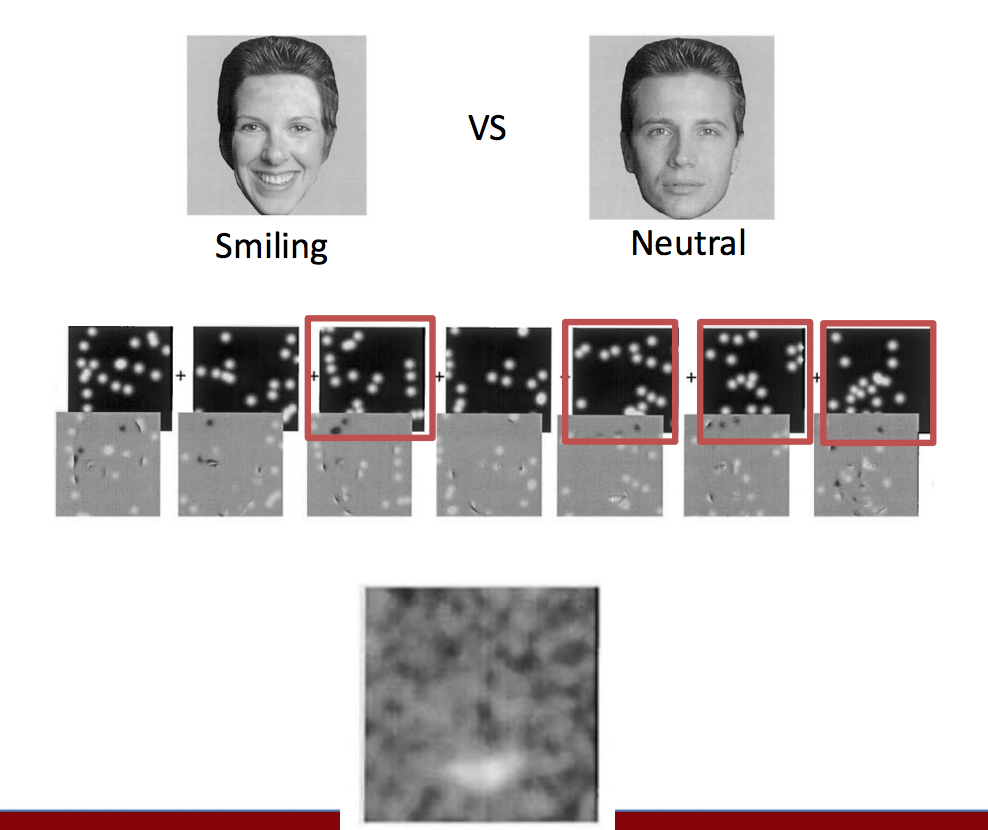
\includegraphics[scale=0.6]{bubblestudy.png}
  \caption{Bubble Method. Source: Lecture 16}
\end{figure}
Another idea is to ask people to annotate images themselves (to simply point out where the important features are). However, this method has no way of easily assuring the quality of these annotations. \\
Crowd-sourced bubble games: online bubble games are similar in nature to the bubble study, but are fun and have monetary rewards for players. Notice that this solves both problems of the above methods -- it is cost effective to have people play, while quality is assured by the reward system of the game. Two examples of games include the following:
\begin{itemize}
\item Peekaboom: Peekaboom was a two-player game in which one player reveals parts of an image, while the other player attempts to guess what the image represents. This game worked well for finding important parts of an image, but was not good for distinguishing between fine-grained classes (since often the important parts of the classes are the same).
\item The Bubbles Game: This game, created by Jia Deng, is an online game in which players are given example images of two classes. Then, a blurred-out image is shown, and the player attempts to guess which class the blurred image belongs to, while revealing only small parts of the image. The less of the image revealed, the more reward is given to the player. This game is much better for finding differences between fine-grained classes, and it led to bubble heatmaps that pinpointed the features that distinguished fine-grained classes, as seen in figure 6.
\begin{figure}[h]
  \centering
  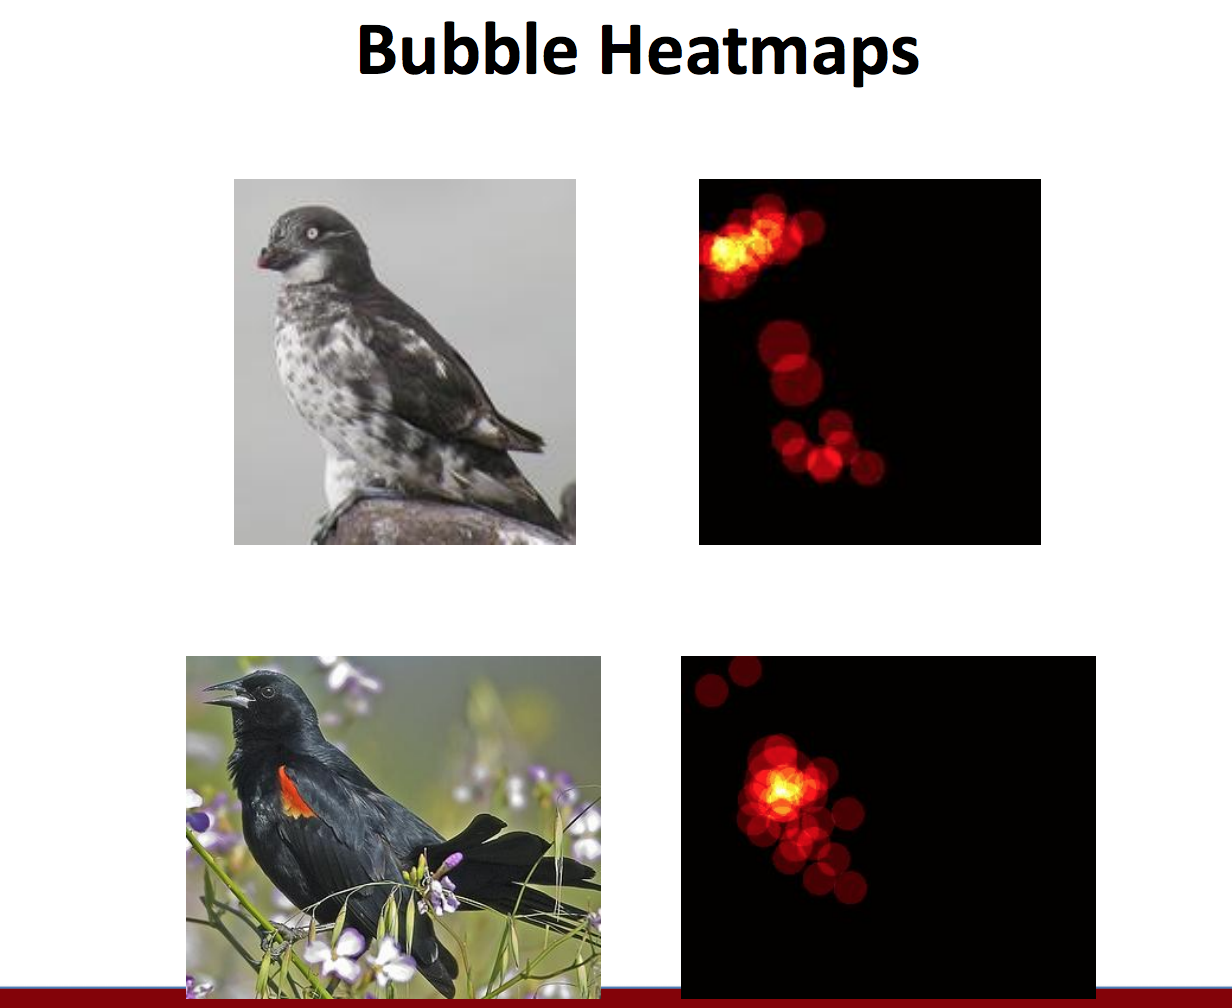
\includegraphics[scale=0.6]{heatmap.png} 
  \caption{Bubble Heatmaps. Source: Lecture 16}
\end{figure}
The creators of the game pooled bubbles from multiple images in a category together and the resulting information was provided to a model, which performed with higher precision than other models at the time.
\end{itemize}
\textbf{References}:\\
{[1]} Everingham, M. and Van-Gool, L. and Williams, C. K. I. and Winn, J. and Zisserman, A. \textit{The PASCAL Visual Object Classes Challenge 2012. (VOC2012) Results}. Retrieved from: http://www.pascal-network.org/challenges/VOC/voc2012/workshop/index.html.

\end{document}

